\documentclass{standalone}
\usepackage{tikz}
\begin{document}
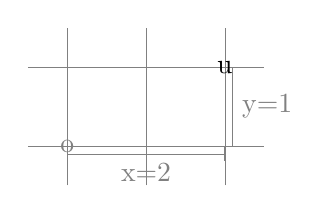
\begin{tikzpicture}
\begin{scope}[help lines]
\draw (-0.5,-0.5) grid (2.5,1.5);
\node at (0,0) {o};
\draw[|-|] (0,-0.1) --node[below]{x=2} (2,-0.1);
\draw[|-|] (2.1,0) --node[right]{y=1} (2.1,1);
\end{scope}

% note the direction of positive x and y
\node at (2,1) {u};

\end{tikzpicture}
\end{document}
